% p38

\section*{Solución propuesta}

\subsection*{1. Identificación del cliente y el servidor}
La solución constará de las siguientes partes:

\begin{itemize}
    \item \textbf{Servidor:} Computador Central (\texttt{CC})
    \item \textbf{Cliente $n$:} Computador del cajero $n$ (\texttt{Cn})
\end{itemize}

Por lo tanto, la arquitectura general de la solución es la siguiente:

\begin{figure}[h]
    \centering
    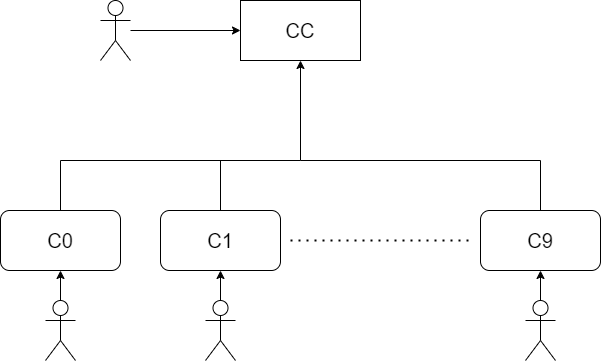
\includegraphics[width=0.6\textwidth]{img/arquitecture.png}
\end{figure}


\subsection*{2. Operaciones y secuencia de intercambio de mensajes}
El sistema contará con cuatro operaciones, con sus consiguientes secuencias de intercambio de mensajes:

\begin{itemize}
    \item \textbf{Apertura:} Cuando el cajero abre la caja.
    \begin{enumerate}
        \item \texttt{Cn} $\rightarrow$ \texttt{CC}: \texttt{\{id,num-caja, hora\}}
        \item \texttt{CC} $\rightarrow$ \texttt{Cn}: 
        \begin{itemize}
            \item \texttt{OK} en caso de que todo haya ido bien.
            \item \texttt{KO} en caso de error (la caja ya está activa, la hora es incorrecta, etc.).
        \end{itemize}
    \end{enumerate}

    \item \textbf{Venta:} Cuando se produce una venta en el cajero.
    \begin{enumerate}
        \item \texttt{Cn} $\rightarrow$ \texttt{CC}: \texttt{\{id, num-caja, hora, importe-total, num-artículos,\\
        id-artículo-0, precio-artículo-0, [...]\}}
        \item \texttt{CC} $\rightarrow$ \texttt{Cn}: 
        \begin{itemize}
            \item \texttt{OK} en caso de que todo haya ido bien.
            \item \texttt{KO} en caso de error (el total no coincide con la suma de los precios de los artículos, la hora es incorrecta, etc.).
        \end{itemize}
    \end{enumerate}
    
    \item \textbf{Cierre:} Cuando el cajero cierra la caja.
    \begin{enumerate}
        \item \texttt{Cn} $\rightarrow$ \texttt{CC}: \texttt{\{id, num-caja, hora, facturación-total, tiempo-total,\\
        artículos-totales\}}
        \item \texttt{CC} $\rightarrow$ \texttt{Cn}: 
        \begin{itemize}
            \item \texttt{OK} en caso de que todo haya ido bien.
            \item \texttt{KO} en caso de error (la caja ya está cerrada, la hora es incorrecta, el tiempo total no coincide con el registro, etc.).
        \end{itemize}
    \end{enumerate}
    
    \item \textbf{Monitorización:} Consulta de estado de una caja.
    \begin{enumerate}
        \item \texttt{CC} $\rightarrow$ \texttt{Cn}: \texttt{\{id, num-caja, hora\}}
        \item \texttt{Cn} $\rightarrow$ \texttt{CC}: 
        \begin{itemize}
            \item \texttt{\{id, num-caja, hora, abierta|cerrada, facturación-total,\\
            tiempo-total, num-artículos\}} en caso de que todo haya ido bien.
            \item \texttt{KO} en caso de error (hora incorrecta, identificador incorrecto, etc.).
        \end{itemize}
    \end{enumerate}
\end{itemize}

Nótese que en todos los mensajes el código de operación va incluído.

\subsection*{3. Protocolo}




\subsection*{4. Formato de los mensajes}




\subsection*{5. Concurrencia}




\subsection*{5. Concurrencia}




\subsection*{6. Nombrado}


